\section{Experiments and discussion}
We evaluate RegionCovOpt on four robot models. We compare the frequency of feasible returns, the costs of accepted motions, and the time each method takes. Matched controls and ablations then separate the contributions of motion construction, regional allocation, and trial generation.

\subsection{Experimental setup}
The benchmark contains twelve scenarios for each of four robot models. We tested fourteen settings in each scenario using seeds 4201, 5209, and 6203, for a total of 2,016 runs. Within each scene--seed pair, all methods use the same geometry, bounds, decoder, first $N_0$ evaluations, and total budget. Acceptance counts cover all runs. Paired cost comparisons use motions accepted for both methods. For timing, we ran three serial repeats on one logical processor.

\begin{center}\begin{minipage}{\linewidth}\centering\small
\TableHere{RegionCovOpt settings shared across scenes. Slot numbering starts at one.}\label{tab:settings}
\begin{tabular}{@{}p{.46\linewidth}p{.48\linewidth}@{}}\toprule
Quantity & Setting\\\midrule
Initial evaluations $N_0$; initialization parent limit $q_0$ & 24; 4\\
Regions $K$; reservation period $H$ & 2; every 4 batches, starting with the first\\
Batch capacity $\lambda$; selected parents $\mu$ & 12; 6\\
Initial scale $\sigma_0$; scale interval & 0.23; $[0.006,0.9]$\\
Coordinate-poll coefficients $(\eta_0,\eta_1)$ & $(0.005,0.4)$\\
Mean, coordinate poll, reserved refresh & First, second and third slot, respectively\\
Archive-centered Gaussian eligibility $\mathcal J_A$ & First five slots, subject to Section~4.2 precedence\\
Total evaluations $B$ & 6,000 (car); 960 (each other robot)\\
\bottomrule\end{tabular}\end{minipage}\end{center}

\subsubsection{Comparison methods and accounting}
We implemented eight controls in C++ under a common interface. They comprise global-best PSO, DE/rand/1/bin, diagonal Gaussian cross-entropy search, full-covariance CMA-ES, multistart finite-difference BFGS, random coordinate polling, uniform sampling, and the earlier regional poll-and-difference method. Decoding and scoring one candidate counts as one evaluation. All budgets include the same 24 initial candidates for a given scene and seed. Planning time includes path-word enumeration, scalar closure calculations, and the planner's feasibility replay. We measure independent verification separately.

PSO uses inertia 0.72984 and two gains of 1.49618. DE uses scale 0.8 and crossover probability 0.9. Cross-entropy search fits the best six of 24 trials with a coordinate standard-deviation floor of 0.025. CMA-ES uses 24 offspring, 12 log-weighted parents, full covariance and step-size adaptation. BFGS takes projected steps on $J+1000V$ with bounded finite differences and backtracking. Each trial used for a difference estimate or a backtracking step counts toward the budget. This BFGS comparison measures the performance of a gradient approximation in the search coordinates shared by all eight controls.

\subsection{Robot models, motion families and validation}
\subsubsection{Autonomous parking} The twelve public \href{https://github.com/libai1943/CommonParking}{CommonParking} cases use their original endpoint headings, vehicle geometry and obstacle polygons. The planner initializes its search from the map and boundary poses. The rear-axle bicycle model has wheelbase 2.8 m. Its state is $(x,y,\theta,v,\phi)$, and its controls are longitudinal acceleration $a=\dot v$ and steering rate $\omega=\dot\phi$. The parking decoder searches nine coordinates. The fourth coordinate divides the direct-connection and intermediate-pose regions at 0.35. Speed, acceleration, steering angle and steering rate have magnitude limits of 2.5 m/s, 1 m/s$^2$, 0.7 rad and 0.5 rad/s, respectively. The rigid rectangular body extends from $-0.929$ to 3.760 m longitudinally and from $-0.971$ to 0.971 m transversely. Dubins~\cite{dubins} characterized shortest forward-only paths under a curvature bound. Reeds and Shepp~\cite{reeds} characterized the corresponding paths when reversal is allowed. Our parking decoder connects oriented poses by signed circular and straight strokes, either directly or through an intermediate pose. Steering transitions occur at rest. The objective is complete maneuver time, including those transitions. The planner checks the rectangular body against a 0.01-m clearance threshold. Recursive midpoint bounds and a sufficient swept-projection shortcut check intersample motion. The independent replay samples at no more than 0.014 m of arc length, reconstructs the rectangle vertices, and checks final position and heading.

\subsubsection{Aerial flight and manipulator motion} The aerial model has three position coordinates and velocities. Its twelve maps contain two, three or four walls with openings at different lateral offsets and elevations. The flight model checks a spherical body of radius 0.22 m against the wall boxes. Each arm case has three joint coordinates and rates and two links of lengths 0.90 and 0.80 m. The arm model places four spheres of radius 0.13 m along each link and measures their clearance from the workspace boxes. The state comprises position and velocity in workspace coordinates for flight and in joint coordinates for the arm. Both models use the three accelerations as controls and integrate each held acceleration exactly. At interval length $\Delta t$ the common position update is
\Eq{spatial}{q_{k+1}=q_k+\Delta t\,v_k+\tfrac12\Delta t^2 a_k.}
\Eq{spatialv}{v_{k+1}=v_k+\Delta t\,a_k.}
The flight and arm decoders both use thirteen coordinates, with a split at 0.45 in the last coordinate. One region uses a velocity profile with zero endpoint velocity and prescribed integrated area, plus coordinate-wise shape changes whose integrated area is removed. The other uses internal knots, with bounded triangular velocity profiles between successive knots. In flight the knots can lie in the specified openings. In joint space they can lift the links, turn the base beyond the requested terminal azimuth, lower the arm and return. Mellinger and Kumar~\cite{snap} obtained quadrotor trajectories by optimizing a polynomial representation. Richter et al.~\cite{uav} exploited a piecewise-polynomial representation for flight through indoor environments. Zhou et al.~\cite{fast} incorporated flight-trajectory generation into replanning in unknown environments. Here the acceleration model allows both search regions to share the same propagation and acceptance tests. For both models the objective adds mean squared controls weighted by 0.01 and squared differences between consecutive controls weighted by 0.002 to the duration. Node clearance is 0.03 m. The violation measure adds the maximum bound excess, the largest dynamics defect, the peak clearance shortfall and its root-mean-square value across nodes. For trials that pass the node tests, open-loop replay subdivides each control interval into twenty steps and checks nonpenetration, state limits and terminal error below $10^{-3}$.

\subsubsection{Articulated reverse docking} The twelve loading bays differ in orientation, access and available staging space. Each task starts at rest in an aisle and ends at rest with the tractor and trailer aligned in a bay. Bay axes range from $44^\circ$ to $88^\circ$ relative to the map axis, on alternating sides of the aisle. All bays have a back wall and both side walls. The other features include a narrow mouth, staggered posts, adjacent occupied berths and a short or long apron. The start can have a nonzero heading. Both forward and reverse motion must occur, and the goal includes both final headings. Each scenario fixes the bay, obstacles, start, and goal.

The coordinates $(x,y)$ locate the tractor's rear axle. The angles $\theta$, $\psi$, and $\phi$ denote the tractor heading, trailer heading, and steering angle, respectively. The tractor wheelbase $L_{\mathrm t}$ and the rear hitch offset $\ell_{\mathrm h}$ are each 1.5 m. The distance $L_{\mathrm r}$ from the hitch to the trailer axle is 3 m. The articulated state augments the tractor position, heading, signed speed and steering angle with the trailer heading. The controls are $a$ and $\omega$, as for the car. With $v$ the signed speed, the heading equations are
\Eq{dhead}{\dot\theta=\frac{v\tan\phi}{L_{\mathrm t}}.}
\Eq{trhead}{\dot\psi=\frac{v\sin(\theta-\psi)-\ell_{\mathrm h}\dot\theta\cos(\theta-\psi)}{L_{\mathrm r}}.}
The tractor rectangle spans $[-0.25,1.8]$ m along the tractor axle frame, with half-width 0.90 m. The trailer rectangle spans $[-1.2,2.25]$ m along the trailer axle frame, with half-width 0.95 m. Both are tested against every oriented obstacle. Speed, acceleration, steering, steering rate and articulation magnitudes are limited to 1.5 m/s, 0.25 m/s$^2$, 0.7 rad, 0.5 rad/s and 1.2 rad.

The regions divide the first coordinate at 0.5. Seven unit-box coordinates choose the side and magnitude of a staging turn, the two bend amplitudes and their skews, and the staging extension. In T04, T08 and T11 a bollard lies ahead of the initial tractor nose. An eighth coordinate sets an initial backward withdrawal of 4.5--11 m, after which the vehicle changes to forward gear for its staging turn. The two regions use opposite staging turns. A bend has normalized arc coordinate $r\in[0,1]$, physical length $S$ and prescribed articulation $\alpha=\theta-\psi$. The amplitude $A$ and skew $k$ determine the articulation profile. Differentiating it with respect to signed distance $s$ and using the hitch equation gives the tractor curvature $\kappa$,
\Eq{alpha}{\alpha(r)=A\sin^2(\pi r)\,[1+k\sin(2\pi r)].}
\Eq{kappa}{\kappa(s)=\frac{\mathrm d\alpha/\mathrm ds+\sin(\alpha)/3}{1+\tfrac12\cos(\alpha)}.}
Both ends of the bend have zero articulation and steering. The integral of the derivative term over the bend vanishes because it is an exact differential and $\alpha(0)=\alpha(1)$. Thus for a prescribed heading change $\delta$ the length is set by
\Eq{length}{S=\frac{\delta}{\displaystyle\int_0^1 \frac{\sin(\alpha(r))}{3(1+\tfrac12\cos(\alpha(r)))}\,\mathrm dr}.}
The decoder constructs a forward bend from the start and an outward bend from the parked pose. A straight terminal stroke translates the outward bend along the bay axis so that both bend ends lie on the same staging line. Resolving their separation onto that line gives the remaining straight distance. Negative required lengths are violations. The rig follows the forward bend and advances to a stop, starting with a backward withdrawal in the three boxed-start tasks. It then reverses along the extension and outward bend into the berth.

Each stroke follows a half-cosine displacement profile with zero speed at both ends. Speed, acceleration, and steering-rate limits determine its duration, with a 1\% allowance. The objective sums the stroke times. The planner checks both rectangular bodies at 97 configurations per stroke against a 0.06-m projection-gap target. The independent verifier reconstructs speed and steering, then integrates the coupled headings from the original start using 400 RK4 steps per stroke. It carries the state across each gear change. Acceptance requires compliance with the physical limits, travel in both directions, terminal error below $10^{-3}$, and at least 0.03 m of body separation at the replay samples.

\subsection{Feasibility, route geometry and paired cost}
\begin{table}[htbp]\centering\small\caption{Independently accepted runs. Each family contributes twelve scenes and three seeds.}\begin{tabular}{lrrrrr}\toprule
Method & Car & Aerial & Arm & Trailer & Total\\\midrule
RegionCovOpt & 34 & 36 & 36 & 36 & 142\\
Particle swarm & 35 & 36 & 34 & 36 & 141\\
Full-covariance CMA-ES & 32 & 36 & 36 & 36 & 140\\
Differential evolution & 36 & 36 & 36 & 36 & 144\\
Gaussian cross-entropy & 32 & 36 & 36 & 36 & 140\\
FD--BFGS & 34 & 36 & 36 & 36 & 142\\
Coordinate polling & 29 & 36 & 35 & 36 & 136\\
Uniform sampling & 36 & 36 & 36 & 36 & 144\\
Poll/difference precursor & 36 & 36 & 36 & 36 & 144\\
\bottomrule\end{tabular}\end{table}
\begin{table}[htbp]\centering\small\caption{Paired primary costs relative to each control. Negative percentages favor RegionCovOpt. A successful motion outranks a failure in the win count.}\begin{tabular}{lrrrrr}\toprule
Control & Joint pairs & Median (\%) & Wins & Losses & Ties\\\midrule
Particle swarm & 139 & -0.23 & 95 & 45 & 4\\
Full-covariance CMA-ES & 139 & -0.43 & 105 & 36 & 3\\
Differential evolution & 142 & -0.42 & 97 & 44 & 3\\
Gaussian cross-entropy & 140 & -3.26 & 122 & 20 & 2\\
FD--BFGS & 140 & -0.32 & 96 & 48 & 0\\
Coordinate polling & 136 & -4.74 & 116 & 26 & 2\\
Uniform sampling & 142 & -6.27 & 125 & 19 & 0\\
Poll/difference precursor & 142 & -0.06 & 79 & 65 & 0\\
\bottomrule\end{tabular}\end{table}
\begin{table}[htbp]\centering\small\caption{Median paired cost change by robot family (percent), computed for runs accepted by both methods.}\begin{tabular}{lrrrr}\toprule
Control & Car & Aerial & Arm & Trailer\\\midrule
Particle swarm & +0.06 & -0.09 & -27.88 & -0.88\\
Full-covariance CMA-ES & -0.01 & -8.81 & -24.64 & +0.12\\
Differential evolution & +2.57 & -8.37 & -27.71 & -0.33\\
FD--BFGS & -3.24 & -24.24 & -0.35 & -0.03\\
\bottomrule\end{tabular}\end{table}

RegionCovOpt returned 142 independently accepted motions in 144 runs. It solved all twelve parking layouts at seed 4201. Its two failures were compact parallel parking P02 at seed 6203 and the two-sided pillar approach P09 at seed 5209. Differential evolution (DE) and uniform sampling each returned 144 accepted motions using the same decoder. With feasibility already common, paired cost reveals how effectively each method used the remaining evaluations.

We calculate the cost change for each pair of accepted motions as
\Eq{paired}{\Delta J=100\left(\frac{J_{\mathrm{RegionCovOpt}}}{J_{\mathrm{control}}}-1\right)\%.}
RegionCovOpt reduced median cost by 0.43\% relative to the original global CMA-ES control across 139 jointly feasible pairs. The largest reduction was 24.64\% in the arm tasks (36 pairs), followed by 8.81\% in flight. Against PSO, the arm reduction was 27.88\% across 34 pairs. Parking costs were close to those of CMA-ES ($-0.01$\%) and PSO ($+0.06$\%). In articulated docking, the median cost was 0.12\% higher than with CMA-ES. DE solved every parking run. On parking pairs accepted by both methods, RegionCovOpt cost 2.57\% more at the median.

Figure~\ref{fig:representative} shows three accepted motions per family at seed 4201. P02 and P09 move forward, reverse and finish in forward gear. P05 starts in reverse and backs into its final pose after a forward maneuver. All three articulated vehicles withdraw, move forward to align and reverse into the bay. The repository includes the complete scene plates and profiles.

\begin{figure*}[p]\centering
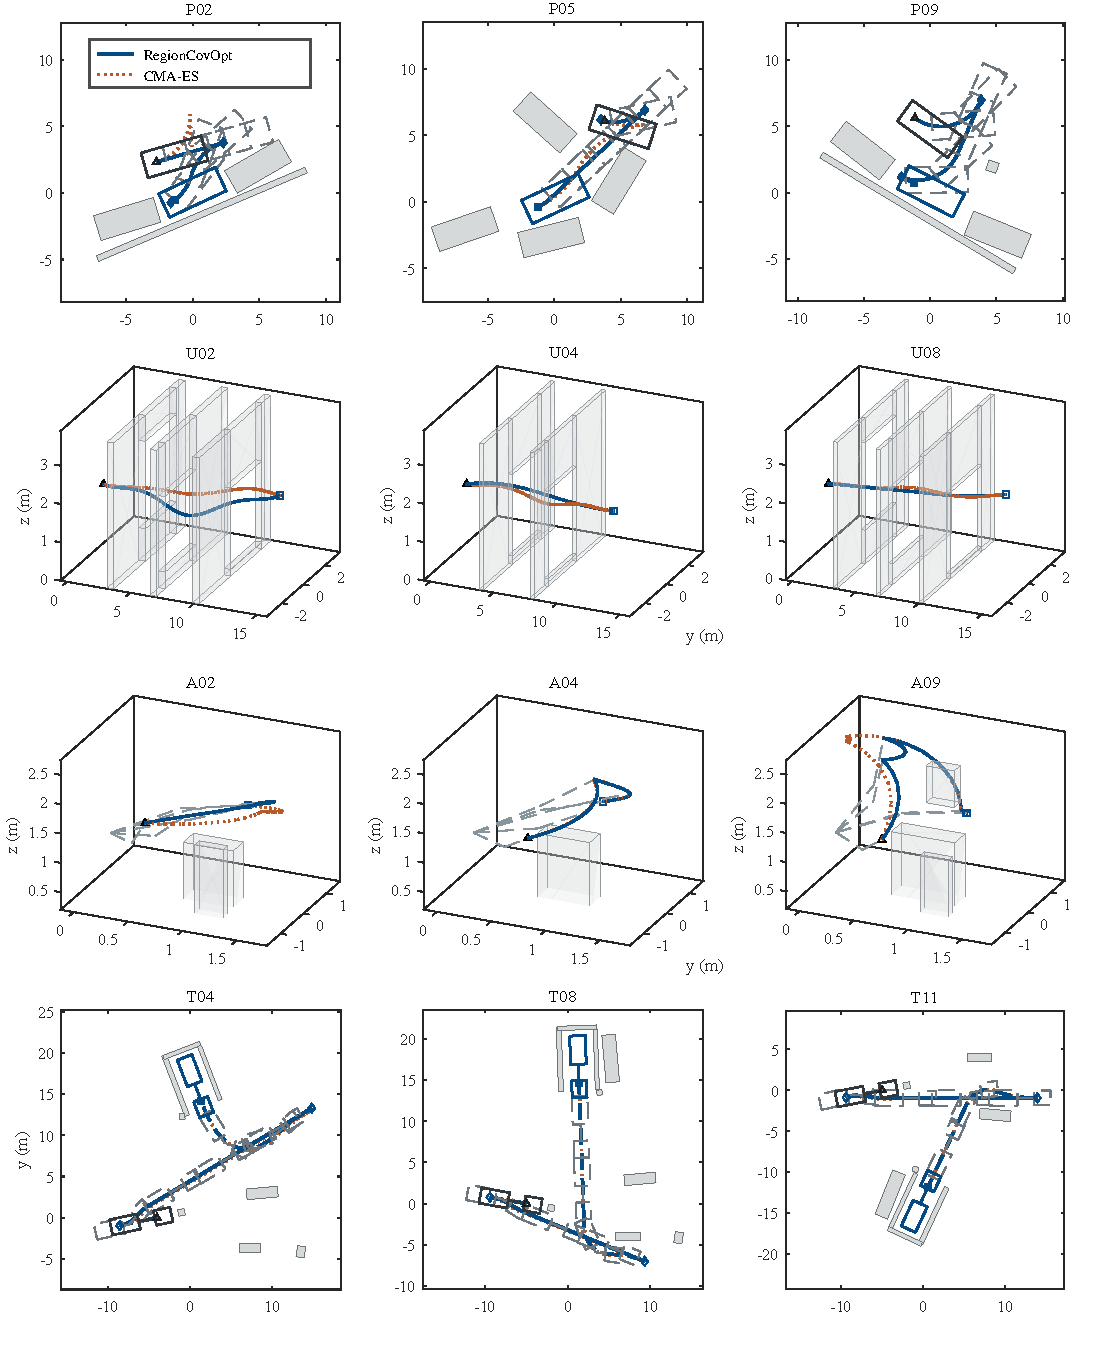
\includegraphics[width=.97\textwidth,height=.85\textheight,keepaspectratio]{../figures/representative.pdf}
\caption{Representative accepted motions at seed 4201. Rows show parking, flight, manipulation and articulated docking. Blue curves show RegionCovOpt and orange dotted curves show global CMA-ES. In the two vehicle rows, solid and dashed blue segments indicate forward and reverse travel. Diamonds mark gear changes and gray dashed rectangles show intermediate footprints. The planar axes use equal physical scales.}\label{fig:representative}
\end{figure*}

\subsection{State and control profiles}
For each scene, the profiles show the lowest-cost RegionCovOpt run that passed independent verification. We selected it from the three prescribed seeds, using the smaller seed to break ties, and reconstructed its controls and states from the initial state to the terminal time $T$. The two vehicle objectives equal $T$. The flight and arm objectives also include control effort and variation. The companion atlas lists the seed, $T$, and $J$ for all 48 scenes.

\begin{figure*}[t]\centering\includegraphics[width=.84\textwidth]{../figures/profile_ground.pdf}
\caption{Best accepted state and control histories for car parking P02 and articulated docking T04. Each column has its own time axis in seconds. Dotted vertical lines mark the onset of travel in the new gear. The angle $\theta$ is the tractor or car heading, $\psi$ the trailer heading and $\phi$ the steering angle.}\label{fig:groundprofiles}\end{figure*}
\begin{figure*}[t]\centering
\includegraphics[width=.84\textwidth]{../figures/profile_spatial.pdf}
\caption{Best accepted histories for aerial flight U04 and manipulator motion A04. The first two rows show configuration and velocity, and the third row shows the applied acceleration. Controls are held over each integration interval.}\label{fig:spatialprofiles}\end{figure*}

Figure~\ref{fig:groundprofiles} illustrates the effect of gear changes on elapsed time. P02 completes its maneuver in 20.99 s. Its signed speed returns to zero for steering changes at rest, so an interval with fixed position can still have nonzero steering rate. T04 starts by withdrawing, moves forward to prepare the approach and reverses into the bay. Forward travel begins at 9.65 s and the final reverse maneuver begins at 43.45 s. Its terminal time is 64.26 s. Figure~\ref{fig:spatialprofiles} shows the independently generated accelerations for U04 and A04. They reach their boundary states in 5.51 s and 2.13 s, respectively. Step changes in the acceleration are retained in the plots, and the state is propagated continuously across those changes.

\subsection{Component and representation ablations}
\begin{table}[htbp]\centering\small\caption{Component ablations. All rows compare the full method against a single change, except the last row which removes the entire special-proposal group.}\begin{tabular}{lrrrrr}\toprule
Variant & Accepted & Joint pairs & Median (\%) & Wins & Losses\\\midrule
Equal batch allocation & 144 & 142 & -0.16 & 97 & 47\\
Diagonal covariance & 144 & 142 & +0.00 & 64 & 77\\
Remove archive poll & 144 & 142 & +0.06 & 49 & 91\\
Remove reserved refresh & 141 & 140 & -0.00 & 74 & 65\\
Gaussian proposals only & 144 & 142 & -0.03 & 85 & 58\\
\bottomrule\end{tabular}\end{table}

Each variant receives the full budget, the same 24 initial members and the same motion representations as RegionCovOpt. Equal allocation spends four of every eight batches in each region. It reverses the alternation phase after four batches so that both regions retain a protected refresh. The diagonal variant removes learned off-diagonal covariances. Two other variants replace either the archive-coordinate poll or the independent reserved draw with the ordinary Gaussian proposal for that slot. The last ablation draws its entire batch about the distribution mean. All comparisons retain feasible alternatives found during the run.

Equal allocation returned two more feasible motions than RegionCovOpt. RegionCovOpt's median cost on their jointly accepted runs was 0.16\% lower. Removing the archive poll yielded 144 accepted motions. The full method cost 0.06\% more at the median on their jointly accepted runs. Dropping covariance cross-terms changed the median cost by less than 0.01\%. Sampling every trial from a Gaussian about the mean yielded 144 accepted motions, with RegionCovOpt 0.03\% lower on jointly accepted pairs. Removing the reserved refresh reduced the count to 141 and had little effect on median cost. The refresh supplies the independent draws in the coverage proof (Appendix B).

On P02 at seed 6203, RegionCovOpt spent 5,200 of 6,000 evaluations in the intermediate-pose region and ended with positive violation. Equal allocation spent 3,004 evaluations there and found its first feasible motion at evaluation 292. On P09 at seed 5209, equal allocation first reached feasibility at evaluation 5,066. Both cases illustrate the risk of concentrating work in the region with the lowest violation before any region has produced a feasible motion.

Direct control sampling yielded zero node-feasible motions in 96 runs. In this experiment, RegionCovOpt and DE each optimized six linearly interpolated control knots per channel and a free duration. We tested each method on all 48 scenes at seed 4201 with the original budgets. Forward integration determined the state history, and a penalty measured terminal error. This encoding increases the search dimension and leaves endpoint satisfaction to the search.

\subsection{Computation time}
\begin{table}[htbp]\centering\small\caption{Minimum process CPU time in seconds across three runs on one logical processor for scene 02 of each family.}\begin{tabular}{lrrrr}\toprule
Method & Car & Aerial & Arm & Trailer\\\midrule
RegionCovOpt & 0.44 & 0.19 & 0.23 & 0.27\\
Particle swarm & 0.38 & 0.19 & 0.20 & 0.28\\
Full-covariance CMA-ES & 0.38 & 0.19 & 0.22 & 0.28\\
Differential evolution & 0.42 & 0.16 & 0.20 & 0.27\\
Gaussian cross-entropy & 0.47 & 0.22 & 0.23 & 0.25\\
FD--BFGS & 0.66 & 0.20 & 0.25 & 0.25\\
Coordinate polling & 0.48 & 0.22 & 0.25 & 0.28\\
Uniform sampling & 0.77 & 0.12 & 0.09 & 0.27\\
\bottomrule\end{tabular}\end{table}

We timed case 02 of each robot on one logical processor and report the minimum process CPU time over three serial runs. Each repeat reproduced the original decision vector. RegionCovOpt took \CarCPU{} s for parking and \DockCPU{} s for articulated docking. PSO and CMA-ES each took 0.38 s for parking and 0.28 s for docking. On the arm case, the corresponding times were 0.23 s for RegionCovOpt, 0.20 s for PSO, and 0.22 s for CMA-ES.

\subsection{Matched controls and contribution attribution}

The matched controls use the same batch size (12), number of log-weighted parents (6), initial scale (0.23), scale limits, and learning rates. Global CMA fits one distribution. The two regional controls fit one distribution per normalized region and allocate batches either equally or by the incumbent/reservation rule. Each control initializes the mean from up to four top-ranked points in its domain and samples about that mean.

\begin{center}\begin{minipage}{\linewidth}\centering\small

\TableHere{Matched controls on the original 144 paired tasks and 128 held-out pairs. $\Delta J$ compares RegionCovOpt with the indicated control, using jointly accepted runs.}

\begin{tabular}{@{}lrrrr@{}}\toprule

Control & \multicolumn{2}{c}{Original} & \multicolumn{2}{c}{Held out}\\

 & Accepted & $\Delta J$ (\%) & Accepted & $\Delta J$ (\%)\\\midrule

RegionCovOpt & 142 & +0.000 & 128 & +0.000\\

Original CMA & 140 & -0.432 & 128 & -0.623\\

Matched global & 141 & -0.171 & 127 & -0.509\\

Regional, equal & 142 & -0.352 & 128 & -0.544\\

Regional, adaptive & 144 & -0.032 & 128 & -0.035\\

DE & 144 & -0.424 & 128 & -1.364\\

Uniform & 144 & -6.270 & 128 & -8.744\\

\bottomrule\end{tabular}\end{minipage}\end{center}

\begin{figure}[tb]
\centering
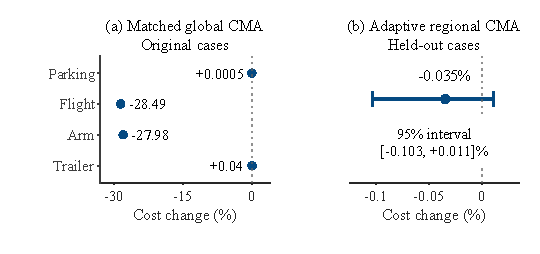
\includegraphics[width=\linewidth]{../figures/attribution.pdf}
\caption{Median paired cost change relative to matched global CMA on the original tasks (a) and adaptively allocated regional CMA on held-out tasks (b). Negative values favor RegionCovOpt. The panels use different horizontal scales. The bar in (b) gives the 95\% scene-cluster bootstrap interval. Only jointly accepted runs enter the comparison.}\label{fig:attribution}
\end{figure}


Figure~\ref{fig:attribution} shows where regional search reduced cost. Flight and manipulation had the largest median gains over matched global CMA. The original-panel median difference narrowed to $-0.032$\% against adaptive regional CMA. The regional controls incorporate both coordinate normalization and region-specific initial means, so this comparison measures their combined effect.

\subsection{Independent selection and held-out task perturbations}

We generated 12 validation tasks and 16 held-out tasks from separate sets of template indices. The perturbations varied the location and size of flight openings, arm goals and obstacles, parking starts and obstacles, and docking starts and aisle geometry. The repository contains the generator, seeds, and inputs.

The original rule led validation with 59 accepted motions in 60 runs. We evaluated five seeds per task and ranked variants first by acceptance count, then by median cost relative to the best accepted candidate for each pair. Removing polling, using diagonal covariance, balancing allocation before feasibility, and combining all three changes yielded 57, 57, 56, and 57 accepted motions, respectively. We fixed the selected rule before testing eight new seeds per held-out task. It and both regional controls returned 128/128 accepted motions. Matched global CMA returned 127/128.

Acceptance therefore favored the full rule on the validation tasks. The held-out cost comparisons below quantify the additional gain over regional CMA.

We estimated a separate 95\% percentile interval for each paired median using 4,000 bootstrap resamples. We resampled whole scenes within each robot family so that the seeds for a scene stayed together. These are marginal intervals for jointly accepted costs.

The held-out median cost change relative to matched global CMA was $-0.509$\% (95\% interval $[-18.400,-0.070]$\%).

The held-out median cost change relative to adaptive regional CMA was $-0.035$\% (95\% interval $[-0.103,0.011]$\%).

The shared initialization produced a motion that passed the planning checks in 125 of 144 original scene--seed pairs within 24 evaluations. This explains much of the early feasibility across optimizers. The budget curves track acceptance by the planner during search. The final cost comparisons use independently verified motions. The repository reports the evaluation count to first feasibility and the complete cost distributions.

\subsection{Representation scope and coverage}

The optimizer transfers across robots through the decoder and evaluator. The parking decoder builds bounded-curvature connections directly or through an intermediate pose. The flight decoder uses ordered rectangular openings, and the arm decoder uses velocity profiles or joint-space knots. The docking decoder uses prescribed gear sequences and aligns the tractor and trailer at the goal. New route branches, joint constraints, or gear sequences may require additional motion families.

At the 960-evaluation budget, each region receives ten independent refreshes after initialization. The probability of reaching a near-optimal motion in these draws depends on how much sampling probability the decoder assigns to that set. Appendix B expresses the bound in terms of that probability. The matched comparisons measure the costs reached at the experimental budget.


Both our C++ implementation of global CMA and pycma 4.5.0 reached objective error below $10^{-8}$ within 12,000 evaluations on all 12 rotated quadratic functions. The problems had dimensions 7, 9, and 13 and condition number $10^3$. Each implementation used its own boundary handling, initial means, and stopping rules. The supplementary records give the final error for each implementation.

\subsection{Planning and independently verified delivery time}

The extended timing test uses cases 02, 05 and 09 of each family, four search rules and three interleaved repeats per rule, giving 144 timed runs on one logical processor. Planning time includes process startup, decoding, scoring and all in-process replay. Independent acceptance is measured separately after reading the returned motion, with task data already loaded. Total wall time is their sum. The table gives median and 90th-percentile wall seconds for RegionCovOpt across the nine runs of each robot; the repository gives all controls and each case's best-of-three process CPU time.

\begin{center}\begin{minipage}{\linewidth}\centering\small

\TableHere{Planning and independent acceptance wall times in seconds. Each entry is median / 90th percentile.}

\begin{tabular}{@{}lrrr@{}}\toprule Robot & Planning & Acceptance & Total\\\midrule

Car & 0.517 / 0.628 & 0.004 / 0.007 & 0.530 / 0.632\\

Flight & 0.212 / 0.273 & 0.037 / 0.045 & 0.249 / 0.309\\

Arm & 0.271 / 0.333 & 0.017 / 0.018 & 0.287 / 0.352\\

Articulated & 0.406 / 0.426 & 0.406 / 0.413 & 0.809 / 0.830\\

\bottomrule\end{tabular}\end{minipage}\end{center}

Independent articulated replay is comparatively expensive because the Python verifier integrates every stroke with 400 RK4 steps and checks both bodies. Its cost should be distinguished from the compiled planner's runtime when assessing a delivered motion. The timings describe open-loop model-based planning and numerical acceptance; hardware execution is a separate validation question.


\section{Conclusion}
RegionCovOpt integrates exploration across parameter regions and local improvement within them. An exploratory trial can immediately improve the best record and redirect subsequent unreserved batches. The same rank and allocation rule apply to each robot through its decoder and evaluator.

Constructing motions that satisfy the endpoint conditions accounted for much of the early feasibility. Regional search then produced its largest cost gains in flight and manipulation. Adaptive regional CMA achieved similar costs to the full method on the held-out tasks. Extending the decoders to new map layouts would let us test whether these task-specific patterns persist.
